% ============================================================
% Aproximación y Proyección Geométrica
% Boyd & Vandenberghe — Capítulos 6 y 8
% Presentación Beamer introductoria
% Curso: Optimización Convexa --- MM-520
% ============================================================
\documentclass[10pt,aspectratio=169]{beamer}

% --- Paquetes ---
\usepackage[utf8]{inputenc}
\usepackage[T1]{fontenc}
\usepackage[spanish]{babel}
\usepackage{amsmath, amssymb, amsthm, mathtools}
\usepackage{tikz}
\usetikzlibrary{calc,arrows.meta,positioning,shapes.geometric,backgrounds,fit}
\usepackage{graphicx}
\usepackage{booktabs}
\usepackage{xcolor}

% --- Tema y colores (mismo estilo que cap4 y cap9) ---
\usetheme{Madrid}
\usecolortheme{seahorse}
\definecolor{accentblue}{RGB}{31,73,125}
\definecolor{accentgreen}{RGB}{46,125,50}
\definecolor{accentred}{RGB}{198,40,40}
\definecolor{accentorange}{RGB}{230,120,30}
\setbeamercolor{frametitle}{bg=accentblue,fg=white}
\setbeamercolor{title}{fg=accentblue}
\setbeamertemplate{navigation symbols}{}
\setbeamertemplate{footline}[frame number]

% --- Datos del documento ---
\title{Aproximación y Proyección Geométrica}
\subtitle{Boyd \& Vandenberghe --- Capítulos 6 y 8}
\author{Optimización Convexa --- MM-520}
\date{\today}

% --- Atajos ---
\newcommand{\R}{\mathbb{R}}
\newcommand{\x}{\mathbf{x}}
\newcommand{\y}{\mathbf{y}}
\newcommand{\xv}{\mathbf{v}}
\newcommand{\xb}{\mathbf{b}}
\newcommand{\bx}{\mathbf{b}}
\newcommand{\xa}{\mathbf{a}}
\newcommand{\z}{\mathbf{z}}
\newcommand{\0}{\mathbf{0}}
\newcommand{\1}{\mathbf{1}}
\newcommand{\res}{\mathbf{r}}
\newcommand{\Sym}{\mathcal{S}}
\newcommand{\Expon}{\operatorname{Exp}}
\newcommand{\norm}[1]{\left\|#1\right\|}
\newcommand{\dom}{\operatorname{dom}}
\newcommand{\epi}{\operatorname{epi}}
\newcommand{\argmin}{\operatorname*{arg\,min}}
\providecommand{\trace}{\operatorname{tr}}

% ============================================================
\begin{document}

% ============================================================
\begin{frame}
  \titlepage
\end{frame}

% ============================================================
\section{Esquema del capítulo}
% ============================================================
\begin{frame}{Esquema}
  \tableofcontents
\end{frame}

% ============================================================
\section{Aproximación por norma y mínima norma}
% ============================================================
\begin{frame}{Aproximación: motivación}
  \begin{block}{Modelo lineal de medición}
    \[
      \y = A\x + \xv, \qquad A\in\R^{m\times n},\ \x\in\R^n,\ \xv\in\R^m.
    \]
  \end{block}
  \begin{itemize}
    \item $\y$: medición observada; $\xv$: error de medición.
    \item ``Implausibilidad'' del error: una \textbf{norma} $\norm{\xv}$.
    \item Dada la medición $\y=\xb$, el valor de $\x$ más plausible es
          el que minimiza $\norm{A\x-\xb}$.
  \end{itemize}
  \vspace{0.3em}
  \begin{alertblock}{Problema de aproximación por norma}
    \begin{equation*}
      \text{minimizar}\quad \norm{A\x-\xb}
      \tag{P$_{\text{norm}}$}
    \end{equation*}
    con $\norm{\cdot}$ cualquier norma de $\R^m$.
  \end{alertblock}
\end{frame}

% ------------------------------------------------------------
\begin{frame}{Forma primal: introduciendo las variables de residuo}
  Reemplazando $\res = A\x - \xb$, el problema (P$_{\text{norm}}$) se
  reescribe como un \textbf{LP / QP según la norma}:
  \[
    \begin{array}{ll}
      \text{minimizar} & \norm{\res} \\
      \text{sujeto a}  & \res = A\x - \xb.
    \end{array}
  \]
  \begin{itemize}
    \item Variable de decisión extendida: $(\x,\res)\in\R^{n+m}$.
    \item Restricción lineal de igualdad: $\res - A\x = -\xb$.
    \item La estructura del problema depende sólo de la norma de $\res$.
  \end{itemize}
\end{frame}

% ------------------------------------------------------------
\begin{frame}{Lecturas frecuentes: geometría, estimación y diseño}
  Tres lecturas equivalentes de (P$_{\text{norm}}$) según el contexto:
  \begin{enumerate}
    \item \textbf{Aproximación geométrica.}\quad
      $A\x^\star$ es el punto del \emph{recorrido} $\mathcal{R}(A)
      \subset \R^m$ más cercano a $\xb$ en la norma $\norm{\cdot}$.
    \item \textbf{Estimación.} \quad
      Dados $y=b$ en el modelo $y=Ax+v$, el $\x^\star$ más plausible
      según $\norm{v}$.
    \item \textbf{Diseño óptimo.} \quad
      $\x$ son variables de diseño, $A\x$ el resultado producido;
      $\x^\star$ aproxima mejor el resultado deseado $\xb$.
  \end{enumerate}

\begin{center}
    % TODO: \includegraphics[width=0.55\textwidth]{<imagen-aquí>}
    \fcolorbox{red}{white}{\parbox[c][3.5cm][c]{0.55\textwidth}{\centering\textcolor{red}{\itshape\bfseries [ imagen aquí ]}}}\\[2pt]
    {\footnotesize \emph{Figura: las tres lecturas equivalentes de la aproximación por norma}.}\\
    {\footnotesize \textcolor{red}{Descripción: ilustrar $\bx\in\R^m$, el recorrido $\R(A)$ como subespacio afín, y $A\x^\star$ como el punto de $\R(A)$ más cercano a $\bx$.}}
  \end{center}
\end{frame}

% ------------------------------------------------------------
\begin{frame}{Ejemplo 1: aproximación euclidiana ($\ell_2$)}
  Norma: $\norm{\cdot = \norm{\cdot}_2}$. Problema:
  \[
    \text{minimizar}\quad \tfrac{1}{2}\norm{A\x-\xb}_2^2.
  \]
  \begin{itemize}
    \item \textbf{Condiciones de optimalidad:} $A^\top(A\x-\xb) = 0$
      --- las \emph{ecuaciones normales}.
    \item \textbf{Solución analítica:} $\x^\star = A^\dagger \xb =
      (A^\top A)^{-1}A^\top \xb$ cuando $A$ tiene rango completo por columnas.
    \item \textbf{En general:} $\x^\star = A^\dagger \xb$, con
      $A^\dagger$ la \emph{pseudoinversa} de Moore--Penrose.
  \end{itemize}
  \begin{block}{}
    Equivale al clásico problema de \emph{mínimos cuadrados}.
  \end{block}
\end{frame}

% ------------------------------------------------------------
\begin{frame}{Ejemplo 2: aproximación \emph{Chebyshev} / \emph{minimax} ($\ell_\infty$)}
  Norma: $\norm{\cdot}_\infty = \max_i |r_i|$. Problema:
  \[
    \text{minimizar}\quad \max_{i=1,\dots,m} |a_i^\top\x - b_i|
    \quad(\text{con } a_i^\top \text{ la } i\text{-ésima fila de } A).
  \]
  \textbf{Formulación como LP:} introducir $t$ que acota las desviaciones:
  \[
    \begin{array}{ll}
      \text{minimizar} & t \\
      \text{sujeto a}  & -t\,\1 \preceq A\x - \xb \preceq t\,\1.
    \end{array}
  \]
  \begin{itemize}
    \item Variables: $(\x,t)\in\R^{n+1}$. Restricciones: $2m$ desigualdades lineales.
    \item $\x^\star$ minimiza el \emph{peor} residuo absoluto.
  \end{itemize}
\end{frame}

% ------------------------------------------------------------
\begin{frame}{Ejemplo 3: suma de residuos absolutos ($\ell_1$)}
  Norma: $\norm{\cdot}_1 = \sum_i |r_i|$. Problema:
  \[
    \text{minimizar}\quad \|A\x-\xb\|_1.
  \]
  \textbf{Formulación como LP:} introducir $y\in\R^m_+$, $y\succeq r$, $y\succeq -r$:
  \[
    \begin{array}{ll}
      \text{minimizar} & \1^\top\y \\
      \text{sujeto a}  & -\y \preceq A\x - \xb \preceq \y.
    \end{array}
  \]
  \begin{itemize}
    \item $\ell_1$ favorece soluciones con \textbf{algunos} residuos grandes y el resto
          exactamente en $0$ (\emph{sparsity} en los residuos).
    \item Robusto frente a valores atípicos comparado con $\ell_2$.
  \end{itemize}
\end{frame}

% ------------------------------------------------------------
\begin{frame}{Aproximación por mínima norma: definición}
  \begin{block}{Problema}
    \begin{equation*}
      \begin{array}{ll}
        \text{minimizar} & \norm{\x} \\
        \text{sujeto a}  & A\x = \xb.
      \end{array}
    \end{equation*}
    \hfill (P$_{\text{LN}}$, least-norm)
  \end{block}
  \begin{itemize}
    \item \emph{Dual} (en cierto sentido) del problema de aproximación por norma:
          intercambia el rol de $\x$ y del residuo $A\x-\xb$.
    \item Factible cuando $\xb\in\mathcal{R}(A)$.
    \item Geométricamente: $\x^\star$ es el punto del conjunto afín
          $\{\x\mid A\x=\xb\}$ más cercano a $\0$ en la norma $\norm{\cdot}$.
  \end{itemize}
\end{frame}

% ------------------------------------------------------------
\begin{frame}{Mínima norma: solución}
  Si $A$ tiene rango completo por filas ($m\ge n$, $\operatorname{rank}(A)=n$):
  \[
    \x^\star = A^\top(AA^\top)^{-1}\xb = A^\dagger\xb.
  \]
  En general, la solución del problema de mínima norma es
  \[
    \x = A^\dagger \xb + (I - A^\dagger A)\z, \qquad \z\in\R^n\text{ arbitrario}.
  \]
  \begin{itemize}
    \item $(I - A^\dagger A)$ es la \emph{proyección ortogonal} sobre el
          espacio nulo de $A$.
    \item La \textbf{única} solución de mínima norma se obtiene tomando $\z=0$.
  \end{itemize}
  \begin{block}{Recuérdese:}
    $A^\dagger = A^\top(A A^\top)^{-1}$ si $A$ rango completo por filas;\\
    $A^\dagger = (A^\top A)^{-1}A^\top$ si rango completo por columnas.
  \end{block}
\end{frame}

% ------------------------------------------------------------
\begin{frame}{Resumen comparativo: las dos caras del mismo cuadro}
  \begin{center}
    \begin{tabular}{lll}
      \toprule
       & \textbf{Aproximación} & \textbf{Mínima norma} \\
       & (sobre $\|\cdot\|$) & (sobre $\|\cdot\|$) \\
      \midrule
      Problema & $\min_\x \|A\x-\xb\|$ & $\min_\x \|\x\|$ \ s.a.\ $A\x=\xb$ \\[0.3em]
      Rol de $\x$ & ajustar el modelo & ser ``lo más pequeño posible'' \\
      Rol de $A\x-\xb$ & residuo a minimizar & debe anularse \\
      Solución ($\ell_2$) & $A^\dagger \xb$ & $A^\top(AA^\top)^{-1}\xb$ \\
      \bottomrule
    \end{tabular}
  \end{center}
  \vspace{0.3em}
  \begin{alertblock}{Idea unificadora}
    Por dualidad, los dos problemas son intercambiables: minimizar la
    norma de un lado es maximizar/dual al otro. La geometría es la misma,
    sólo cambia el papel de cada variable.
  \end{alertblock}
\end{frame}

% ============================================================
\section{Aproximación regularizada}
% ============================================================
\begin{frame}{¿Por qué regularizar?}
  En la práctica $A\x=\xb$ raramente es soluble, o $A^\top A$ está mal
  condicionada y $\x^\star = (A^\top A)^{-1}A^\top \xb$ explota.
  \begin{itemize}
    \item \textbf{Sobre-ajuste:} LS puro se ajusta al ruido de $\xb$ y pierde poder de generalización.
    \item \textbf{Multicolinealidad:} con $A^\top A$ singular o casi, $A^\dagger$ amplifica errores.
    \item \textbf{Mal condicionamiento:} $\kappa(A^\top A)=\kappa(A)^2\gg 1$.
  \end{itemize}
  \begin{alertblock}{Idea central}
    Añadir al objetivo un \textbf{término de penalización} $\lambda R(\x)$ que
    ``empuje'' a $\x$ hacia un comportamiento deseado (pequeño, disperso, suave\ldots).
  \end{alertblock}
\end{frame}

% ------------------------------------------------------------
\begin{frame}{Regularización de Tikhonov ($\ell_2$)}
  \begin{equation*}
    \begin{array}{ll}
      \text{minimizar} & \norm{A\x - \xb}_2^2 + \lambda \norm{\x}_2^2 \\
      \text{} & \lambda > 0 \text{ (parámetro de regularización)}.
    \end{array}
  \end{equation*}
  \begin{itemize}
    \item $\lambda\to 0$: recupera mínimos cuadrados.
    \item $\lambda\to\infty$: domina el segundo término, $\x^\star\to 0$.
    \item \textbf{Condiciones de optimalidad:}
      $(A^\top A + \lambda I)\,\x = A^\top\xb$.
    \item \textbf{Solución:} $\x^\star = (A^\top A + \lambda I)^{-1}A^\top\xb$.
    \item Resuelve el mal condicionamiento \emph{siempre} ($A^\top A+\lambda I\succ 0$).
  \end{itemize}
  \begin{block}{Nombres clásicos}
    Estadística: \emph{ridge regression}. Visión por computador y
    reconstrucción de imágenes: \emph{Tikhonov}.
  \end{block}
\end{frame}

% ------------------------------------------------------------
\begin{frame}{Otras penalizaciones frecuentes}
  \begin{center}
    \begin{tabular}{lll}
      \toprule
      Nombre & Objetivo & Efecto \\
      \midrule
      Ridge / Tikhonov & $\|A\x-\xb\|^2 + \lambda\|\x\|_2^2$ & $\x$ pequeño global \\
      Lasso & $\|A\x-\xb\|^2 + \lambda\|\x\|_1$ & $\x$ disperso (sparse) \\
      Elastic net & $\|A\x-\xb\|^2 + \alpha\|\x\|_2^2 + \beta\|\x\|_1$ & disperso + estable \\
      Total variation & $\|A\x-\xb\|^2 + \lambda\operatorname{TV}(\x)$ & $\x$ suave a trozos \\
      \bottomrule
    \end{tabular}
  \end{center}
  \begin{itemize}
    \item \textbf{Selection de $\lambda$:} validación cruzada, cota sobre $\|\x\|$,
          discrepancia (Morozov), curvas-L.
    \item \textbf{Forma en norma:} cualquier $\phi(\x)$ convexa, monótona en
          $\|\x\|$, entrega un regularizador.
  \end{itemize}
\end{frame}

% ------------------------------------------------------------
\begin{frame}{Ajuste por función de penalización: (P$_\phi$)}
  En lugar de una norma, se puede usar una \emph{función de penalización}:
  \[
    \begin{array}{ll}
      \text{minimizar} & \phi(r_1) + \cdots + \phi(r_m) \\
      \text{sujeto a}  & \res = A\x - \xb.
    \end{array}
    \qquad\text{(P}_\phi\text{)}
  \]
  con $\phi:\R\to\R$ \textbf{convexa}. Tres elecciones clásicas:
  \[
    \begin{array}{ll}
      \phi(u)=u^2            & \text{(cuadrática, sensible a outliers)}, \\[0.3em]
      \phi(u)=\max\{0,|u|-a\} & \text{(deadzone-lineal: ignora $|u|\le a$)},\\[0.3em]
      \phi(u)=\begin{cases}
                  -(a^2/2)\log(1-(u/a)^2) & |u|<a, \\
                  +\infty                 & |u|\ge a
              \end{cases} & \text{(log-barrera: fuerza $|u|<a$)}.
    \end{array}
  \]
  La forma de $\phi$ controla la \emph{distribución} del residuo.

\begin{center}
    % TODO: \includegraphics[width=0.55\textwidth]{<imagen-aquí>}
    \fcolorbox{red}{white}{\parbox[c][3.5cm][c]{0.55\textwidth}{\centering\textcolor{red}{\itshape\bfseries [ imagen aquí ]}}}\\[2pt]
    {\footnotesize \emph{Figura: gráfica de las tres $\phi$: cuadrática, deadzone-lineal, log-barrera}.}\\
    {\footnotesize \textcolor{red}{Descripción: mostrar cómo cada $\phi$ se comporta cerca y lejos de $0$; comparar con la curva $|u|$ y $u^2$.}}
  \end{center}
\end{frame}

% ============================================================
\section{Aproximación paramétrica de distribuciones}
% ============================================================
\begin{frame}{Estimación paramétrica: hipótesis}
  \begin{block}{Supuesto}
    Los datos $x_1,\dots,x_n\in\R$ son i.i.d. según una densidad
    \[
      p(x;\theta), \qquad \theta\in\Theta\subset\R^p.
    \]
    La \emph{familia paramétrica} $\{p(\,\cdot\,;\theta)\}_{\theta\in\Theta}$ es conocida
    salvo el valor de $\theta$.
  \end{block}
  \begin{itemize}
    \item \emph{Ejemplos:} Gaussiana $\mathcal{N}(\mu,\sigma^2)$,
          exponencial $\Expon(\lambda)$, Bernoulli, Poisson, mezcla finita.
    \item \textbf{Objetivo:} a partir de los datos, estimar $\theta$.
  \end{itemize}
\end{frame}

% ------------------------------------------------------------
\begin{frame}{Estimación por máxima verosimilitud (ML)}
  \begin{block}{Función de verosimilitud y log-verosimilitud}
    \[
      L(\theta) = \prod_{i=1}^n p(x_i;\theta), \qquad
      \ell(\theta) = \log L(\theta) = \sum_{i=1}^n \log p(x_i;\theta).
    \end{equation*}
  \end{block}
  \begin{itemize}
    \item El estimador de máxima verosimilitud (ML/MLE) es
      $\displaystyle \theta_{\mathrm{ML}} = \arg\max_\theta L(\theta)
       = \arg\min_\theta\, -\ell(\theta)$.
    \item $-\ell$ es \emph{suma de funciones} de la densidad $p(\,\cdot\,;\theta)$ en cada dato:
          encaja como un problema de \emph{penalización} (P$_\phi$).
  \end{itemize}
  \begin{alertblock}{Caso Gaussiano}
    Con $p(x;\mu,\sigma^2) = \tfrac{1}{\sqrt{2\pi\sigma^2}}\,e^{-(x-\mu)^2/(2\sigma^2)}$,
    $\theta = (\mu,\sigma^2)$ y el negativo de la log-verosimilitud
    \[
      -\ell(\mu,\sigma^2)=\tfrac{1}{2\sigma^2}\sum_i (x_i-\mu)^2 + \tfrac{n}{2}\log(2\pi\sigma^2),
    \]
    cuya minimización da
    $\hat\mu=\tfrac1n\sum_i x_i$ y
    $\hat\sigma^2=\tfrac1n\sum_i (x_i-\hat\mu)^2$.
  \end{alertblock}
\end{frame}

% ------------------------------------------------------------
\begin{frame}{Ejemplo discreto: MLE para una \emph{Poisson}($\lambda$)}
  \centering
  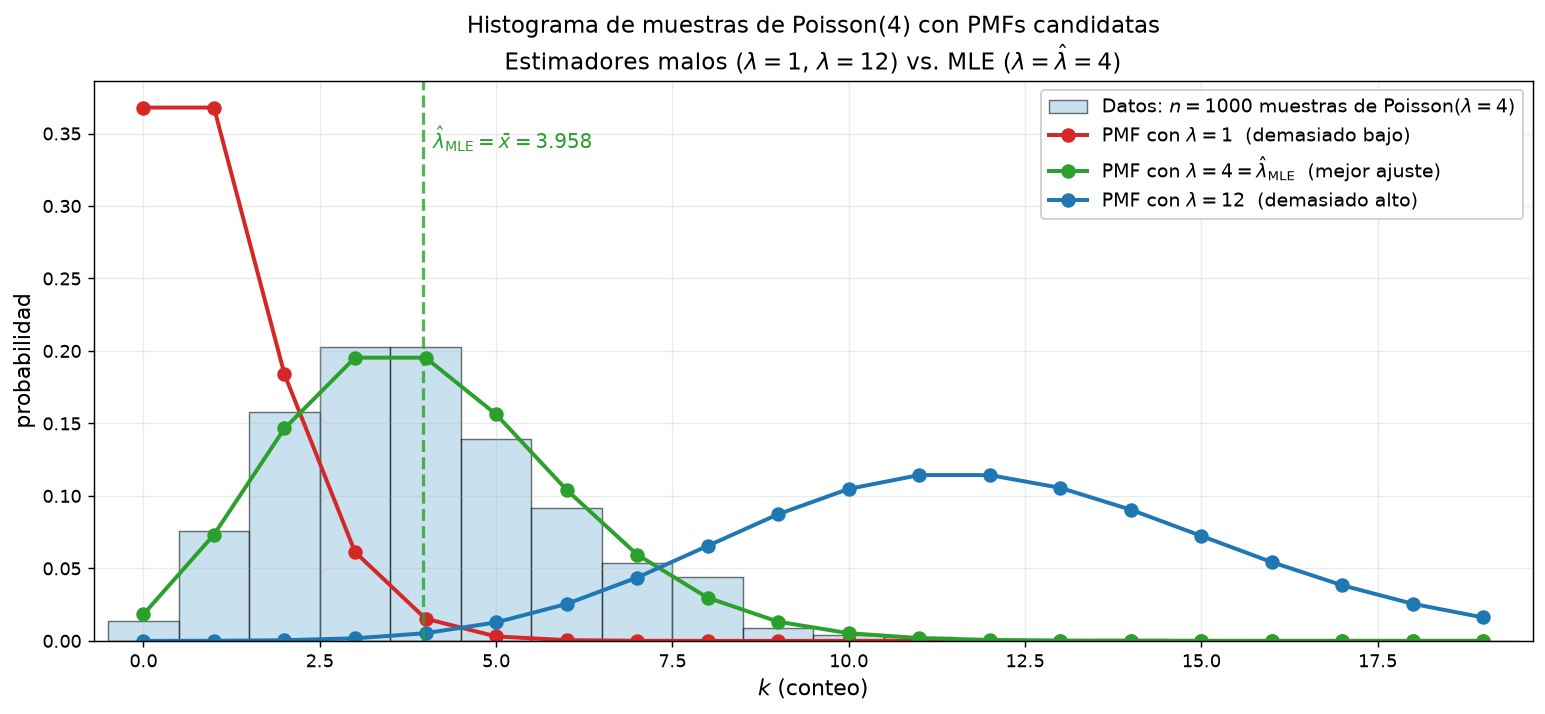
\includegraphics[width=0.82\textwidth]{cap_aproximacion_y_proyeccion_images/poisson_mle_histogram.jpg}

  \vspace{0.4em}
  \begin{footnotesize}
    $n=1000$ muestras i.i.d.\ de Poisson($\lambda^\star = 4$);
    $\hat\lambda_{\mathrm{MLE}} = \bar x = 3.958 \approx 4$.
    De $\lambda\in\{1,12\}$ sólo $\lambda = 4 = \hat\lambda_{\mathrm{MLE}}$ ajusta el histograma.
  \end{footnotesize}
\end{frame}

% ------------------------------------------------------------
\begin{frame}{Estimación MAP = aproximación regularizada}
  \begin{block}{Estimador MAP (máximo a posteriori)}
    \[
      \theta_{\mathrm{MAP}} \;=\; \arg\max_\theta\;
        \underbrace{p(\theta)}_{\text{priori}}\cdot
        \underbrace{p(x_1,\dots,x_n\mid\theta)}_{\text{verosimilitud}}
      \;=\; \arg\min_\theta\;
        \bigl[-\log p(x;\theta)\bigr] \;+\; \bigl[-\log p(\theta)\bigr].
    \]
  \end{block}
  \begin{itemize}
    \item Es la \textbf{fusión de dos ingredientes convexos}:
          likelihood y priori.
    \item \textbf{Caso clave:} priori Gaussiano
          $\theta\sim\mathcal{N}(\0,\tau^2 I)$ $\Rightarrow$
          $-\log p(\theta)=\tfrac1{2\tau^2}\norm{\theta}_2^2 + \text{cte}$.
          MAP = \emph{Tikhonov} con $\lambda = 1/\tau^2$.
  \end{itemize}
  \begin{alertblock}{Re-encuadre como problema convexo}
    ML: $\min_\theta -\sum_i\log p(x_i;\theta)$. \\
    MAP: $\min_\theta -\sum_i\log p(x_i;\theta) + \Omega(\theta)$
    (penalización por la priori).
  \end{alertblock}
\end{frame}

% ============================================================
\section{Una aplicación clásica: optimización de portafolios (Markowitz)}
% ============================================================
\begin{frame}{Motivación con datos reales: dos rutas para comprar USD}
  \begin{itemize}
    \item En la práctica hay \textbf{dos activos} para hacerse de USD en
          Honduras: la compra \emph{bancaria} (precio estable, LPS Dólar
          --Compra / --Venta) y la compra \emph{vía P2P} con USDT (precio
          de mercado, volátil, USDT P2P--Mejor venta).
    \item Pregunta natural: ¿cuándo conviene cada ruta? ¿Se pueden mezclar
          para mejorar el \emph{precio efectivo}?
    \item Es exactamente el problema de Markowitz: dos activos correlacionados
          con perfiles distintos de retorno esperado ($\mu$) y riesgo
          ($\Sigma$).
    \item Los datos (ago 2025 -- jul 2026) muestran: el banco es estable pero
          caro, el P2P es más barato en media pero mucho más volátil.
          Combinarlos reduce varianza sin sacrificar precio promedio.
  \end{itemize}
  \begin{center}
    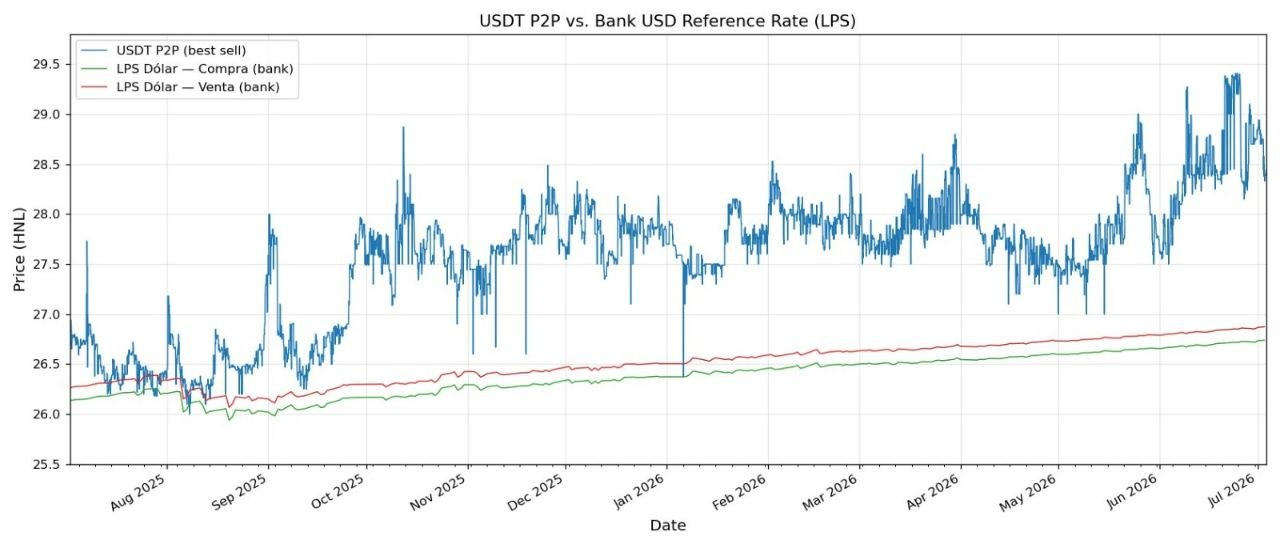
\includegraphics[width=0.78\textwidth]{cap_aproximacion_y_proyeccion_images/usdt_p2p_vs_banco_lps.jpg}
  \end{center}
\end{frame}

% ------------------------------------------------------------
\begin{frame}{Motivación: diversificación y riesgo}
  \begin{itemize}
    \item Un inversionista elige pesos $w_i\ge0$ sobre $n$ activos con retornos
          aleatorios $r_i$, $\sum_i w_i = 1$ (cartera autofinanciada).
    \item Retorno y riesgo del portafolio (asumiendo retornos independientes
          del período):
          \[
            R(w) \;=\; \mu^{\top}\! w, \qquad
            \sigma^2(w) \;=\; w^{\top}\Sigma w,
          \]
          con $\mu\in\R^n$ los retornos esperados y $\Sigma\succ0$ la matriz de
          covarianzas.
    \item \textbf{Idea clave de Markowitz (1952):} la varianza del
          portafolio es menor que el promedio ponderado de las varianzas
          individuales, siempre que los activos no estén perfectamente
          correlacionados.
          \[
            \sigma^2(w) \;=\; \sum_i w_i^2\,\sigma_i^2
                            \;+\; \sum_{i\ne j} w_i w_j\,\sigma_{ij}
                            \;<\; \sum_i w_i\,\sigma_i^2
                            \quad\text{(si }\sigma_{ij}<0\text{ para algún par)}.
          \]
    \item Por tanto se puede \emph{reducir el riesgo sin sacrificar
          rendimiento esperado}, eligiendo pesos que exploten la covarianza.
  \end{itemize}
\end{frame}

% ------------------------------------------------------------
\begin{frame}{El modelo de media--varianza (Markowitz, 1952)}
  \textbf{Datos:} $\mu\in\R^n$, $\Sigma\in\R^{n\times n}$ ($\Sigma\succ0$),
  presupuesto $W=1$, restricción de no--venta corta opcional
  $w\ge0$ (o $\ge -w_{\max}$, etc.).
  \[
    \boxed{
      \begin{array}{rl}
        (P_{\mathrm{MV}}) \quad & \min\limits_{w\in\R^n}\; w^{\top}\Sigma\, w \\[2pt]
                               & \text{s.t.}\quad \mu^{\top} w \;\ge\; R_{\min}, \\[2pt]
                               & \phantom{\text{s.t.}}\quad \mathbf{1}^{\top} w \;=\; 1.
      \end{array}}
  \]
  Variantes equivalentes (todas convexas):
  \begin{itemize}
    \item Minimizar $\sigma^2(w)$ para una \emph{rentabilidad objetivo} $R_{\min}$.
    \item Maximizar $\mu^{\top} w - \lambda\,w^{\top}\Sigma w$ para
          $\lambda>0$ dado (aversión al riesgo).
    \item Minimizar $\sigma^2(w)$ en la \emph{forma estándar} de QP
          \[
            \begin{array}{rl}
              \min\limits_{w}\;& w^{\top}\Sigma w \\
              \text{s.t.}\;& A w = b,\quad G w \le h
            \end{array}
          \]
          que \emph{es exactamente} un problema de la familia
          $(\mathrm{QP})$ de Boyd--Vandenberghe.
  \end{itemize}
  \begin{exampleblock}{Relación con lo anterior}
    La forma dual de $(P_{\mathrm{MV}})$ es una \emph{aproximación
    regularizada} (Tikhonov) sobre los retornos:
    $\min_w\;\|\Sigma^{1/2}w\|^2$ controlado por $\mu$ ---
    el mismo aparato convexo de $\ell_2$ y $\phi$.
  \end{exampleblock}
\end{frame}

% ------------------------------------------------------------
\begin{frame}{Frontera eficiente}
  \begin{columns}[T]
    \begin{column}{0.55\textwidth}
      \begin{itemize}
        \item Al resolver $(P_{\mathrm{MV}})$ para cada valor de
              $R_{\min}\in[\mu_{\min},\mu_{\max}]$ se obtiene la
              \textbf{frontera eficiente}: el conjunto de portafolios
              con menor varianza para cada nivel de retorno esperado.
        \item En el plano $(\sigma,R)$ la frontera es una hipérbola
              que abre hacia la derecha (las dos ramas superior e
              inferior son simétricas; sólo la superior es eficiente).
        \item \textbf{Capital Market Line (CML):} al añadir un activo
              libre de riesgo con retorno $r_f$, la mejor combinación
              se obtiene en la recta tangente a la frontera que pasa
              por $(0,r_f)$:
              \[
                R_P \;=\; r_f + \frac{\mu_M - r_f}{\sigma_M}\,\sigma_P.
              \]
        \item La pendiente $(\mu_M-r_f)/\sigma_M$ es el \emph{precio
              de mercado del riesgo}.
      \end{itemize}
    \end{column}
    \begin{column}{0.42\textwidth}
      \fcolorbox{red}{white}{\parbox[c][5.5cm][c]{\linewidth}{\centering\color{red}\itshape\bfseries [ esquema: $(\sigma,R)$ con\\frontera eficiente\\y CML ]}}
    \end{column}
  \end{columns}
\end{frame}

% ------------------------------------------------------------
\begin{frame}{Convexidad y resolución}
  \begin{itemize}
    \item $(P_{\mathrm{MV}})$ es un \textbf{QP convexo}:
      \begin{itemize}
        \item objetivo: forma cuadrática $w^{\top}\Sigma w$ con
              $\Sigma\succ0$ $\Rightarrow$ fuertemente convexa;
        \item restricciones: lineales (afines) $\Rightarrow$ conjunto
              factible convexo.
      \end{itemize}
    \item \emph{Por tanto} existe un único óptimo y los KKT son
          \emph{suficientes}. Se resuelve en milisegundos con métodos
          de punto interior para $n$ moderado ($\sim10^3$ activos).
    \item Markowitz desarrolló el \textbf{método de la línea crítica}
          (1956), un algoritmo de programación cuadrática que traza
          toda la frontera eficiente cambiando $R_{\min}$ entre
          restricciones activas.
    \item Métodos generales aplicables: gradiente proyectado,
          Newton truncado, \emph{ADMM} para problemas
          separables, solvers de barrera modernos.
  \end{itemize}
  \begin{block}{Críticas conocidas (y por qué importa la convexidad)}
    \begin{itemize}
      \item \emph{Error maximization:} pequeños errores en
            $\hat\mu$, $\hat\Sigma$ producen cambios enormes en $w^\star$.
      \item Sin $w\ge0$, la solución puede ser altamente apalancada
            (largos en unos activos, cortos en otros); en la práctica
            se impone $w\ge0$ (o cotas por posición).
      \item La covarianza empírica subestima las correlaciones reales
            en crisis; alternativas: shrinkage (Ledoit--Wolf),
            Black--Litterman, jerarquía de riesgo (HRP).
    \end{itemize}
  \end{block}
\end{frame}

% ============================================================
\section{Aproximación no paramétrica de distribuciones}
% ============================================================
\begin{frame}{Estimación no paramétrica: idea}
  \begin{itemize}
    \item \textbf{No asumimos una forma paramétrica} $p(x;\theta)$.
    \item Objetivo: estimar la densidad $p(x)$ en cada $x$ (o una
          función desconocida $f:\R\to\R$) \emph{sólo} a partir de
          datos, sin conocimiento previo de su forma.
    \item Toda la información está en los datos: ``\emph{let the data speak}''.
  \end{itemize}
  \vspace{0.3em}
  \begin{block}{Resumen de los tres métodos que veremos}
    \begin{enumerate}
      \item Estimación por \emph{histogramas}.
      \item Estimación por \emph{kernel} (KDE).
      \item Estimación por \emph{$k$-vecinos más cercanos} ($k$-NN).
    \end{enumerate}
  \end{block}
\end{frame}

% ------------------------------------------------------------
\begin{frame}{Estimación por histogramas}
  Dividir el rango en $M$ celdas de ancho $h$ y contar cuántos datos caen en cada una.
  \[
    \hat p_{\text{hist}}(x) \;=\; \frac{1}{n h}\,\#\{i\mid x_i \text{ cae en la celda que contiene } x\}.
  \]
  \begin{itemize}
    \item \textbf{Ventaja:} extremadamente simple, rápida.
    \item \textbf{Desventaja:} discontinua en los bordes de celda,
          depende de $M$ y de dónde se cortan las celdas.
    \item Elección del ancho $h$: sesgo vs.\ varianza (ancho pequeño
          $\to$ alta varianza; ancho grande $\to$ alto sesgo).
  \end{itemize}
\end{frame}

% ------------------------------------------------------------
\begin{frame}{Estimación por kernel (KDE)}
  \begin{block}{Estimador de Parzen--Rosenblatt}
    \[
      \hat p(x) \;=\; \frac{1}{n h}\sum_{i=1}^n K\!\left(\frac{x - x_i}{h}\right),
    \]
    donde $K:\R\to\R_+$ es un \emph{kernel} (e.g.\ Gaussiano, Epanechnikov,
    triangular, uniforme) con $\int K = 1$.
  \end{block}
  \begin{itemize}
    \item \emph{Intuición:} poner una ``campana'' $K$ sobre cada dato
          y promediar.
    \item Continuidad y suavidad heredadas de $K$.
    \item \textbf{Ancho de banda $h$:} controla el tradeoff sesgo/varianza
          --- usualmente $h\propto n^{-1/5}$ para datos en 1D.
  \end{itemize}
\end{frame}

% ------------------------------------------------------------
\begin{frame}{Estimación por $k$-vecinos más cercanos}
  Idea: estimar la densidad en $x$ por la \emph{frecuencia local}
  alrededor de $x$, medida con la métrica de los $k$ vecinos más próximos.
  \[
    \hat p(x) \;=\; \frac{k/n}{\operatorname{vol}\bigl(B(x,\,r(x))\bigr)},
    \qquad
    r(x) \;=\; \text{distancia al }k\text{-ésimo vecino más cercano de } x.
  \]
  \begin{itemize}
    \item \emph{Análoga en clasificación:} asignar a $x$ la clase
          mayoritaria de sus $k$ vecinos más cercanos.
    \item \textbf{Ventaja:} no asume forma para la densidad; ``adaptativa''
          (en regiones con pocos datos, $r$ crece).
    \item \textbf{Costo:} requiere $k$-NN queries --- $O(n\log n)$ con
          árboles (KD-trees, ball-trees), $O(nd)$ lineales.
  \end{itemize}
\end{frame}

% ============================================================
\section{Proyección sobre un conjunto convexo}
% ============================================================
\begin{frame}{Proyección: definición}
  \begin{block}{Proyección euclidiana de $\x_0$ sobre $C$}
    \begin{equation*}
      \Pi_C(\x_0) \;=\; \arg\min_{\x\in C}\, \tfrac{1}{2}\norm{\x - \x_0}_2^2.
    \end{equation*}
  \end{block}
  \begin{itemize}
    \item Si $C$ es \textbf{convexo cerrado} no vacío, el problema tiene
          \emph{única} solución (convexidad + función objetivo estrictamente
          convexa).
    \item Si $C=\emptyset$: no hay proyección. Si $C$ no convexo: la
          proyección puede no ser única o no existir.
  \end{itemize}
\end{frame}

% ------------------------------------------------------------
\begin{frame}{Caracterización variacional de la proyección}
  $\x^\star = \Pi_C(\x_0)$ \emph{si y sólo si} se cumple la
  \textbf{condición variacional}:
  \[
    (\x_0 - \x^\star)^\top(\x - \x^\star) \;\le\; 0
    \qquad\forall\,\x\in C.
  \]
  \begin{itemize}
    \item Lectura geométrica: el vector $\x^\star - \x_0$ es \emph{normal}
          a $C$ en el punto $\x^\star$, apuntando hacia adentro.
    \item Equivale a decir que $\x_0 - \x^\star$ pertenece al cono normal
          $N_C(\x^\star)$.
  \end{itemize}
  \begin{alertblock}{Consecuencia clave}
    La condición variacional es el análogo convexo de las
    \emph{condiciones KKT} para problemas con un único conjunto factible
    convexo.
  \end{alertblock}
\end{frame}

% ------------------------------------------------------------
\begin{frame}{Ejemplos clásicos de proyección}
  \begin{enumerate}
    \item \textbf{Hiperplano} $H = \{\x\mid \xa^\top\x = b\}$:
      \[
        \Pi_H(\x_0) \;=\; \x_0 + \tfrac{b-\xa^\top\x_0}{\|\xa\|_2^2}\,\xa.
      \]
    \item \textbf{Half-space} $H^- = \{\x\mid \xa^\top\x \le b\}$:
      $\Pi_{H^-}(\x_0)$ = proyección sobre $H$ si $\xa^\top\x_0 \le b$; en otro caso $= \x_0 + \tfrac{b-\xa^\top\x_0}{\|\xa\|_2^2}\xa$.
    \item \textbf{Bola euclidiana} $B=\{c\}\oplus r\mathbb{B}$:
      \[
        \Pi_B(\x_0)=\begin{cases}
                      \x_0 & \text{si } \|\x_0-c\|_2\le r,\\[0.2em]
                      c + r\,\dfrac{\x_0-c}{\|\x_0-c\|_2} & \text{si } \|\x_0-c\|_2>r.
                    \end{cases}
      \]
    \item \textbf{Caja} $C = \{\x\mid \text{\textbf l}\preceq\x\preceq\text{\textbf u}\}$: $\Pi_C(\x_0)$
      se aplica coordenada a coordenada,
      $\bigl[\Pi_C(\x_0)\bigr]_i = \min(u_i,\,\max(\ell_i,\,x_{0,i}))$.
  \end{enumerate}
\end{frame}

% ------------------------------------------------------------
\begin{frame}{Proyección sobre conos y la PSD}
  \begin{itemize}
    \item \textbf{Cono $K$:} la proyección sobre un cono convexo cerrado
          $K$ satisface $\Pi_K(\x_0) = (\x_0 - \Pi_{K^\star}(\x_0))$ (descomposición de Moreau).
    \item \textbf{Cono no negativo} $K=\R_+^n$:
      $\Pi_{\R_+^n}(\x_0)$ recorta a $0$ las coordenadas negativas.
    \item \textbf{Cono PSD} $\Sym_+^n = \{S\mid S=S^\top,\ S\succeq 0\}$:
      la proyección euclidiana de $\x_0$ sobre $\Sym_+^n$ es
      $V\,\operatorname{diag}(\lambda_+)\,V^\top$, donde $\x_0 = V\,\operatorname{diag}(\lambda)\,V^\top$
      es la descomposición propia y $\lambda_+ = \max(\lambda,\,0)$.
    \item \textbf{Cajas y poliedros:} en general la proyección sobre un
          poliedro se reduce a un \emph{QP} (cuadrático convexo).
  \end{itemize}
\end{frame}

% ============================================================
\section{Distancia entre conjuntos y separación}
% ============================================================
\begin{frame}{Distancia entre dos conjuntos convexos}
  \begin{block}{Distancia euclidiana entre $C$ y $D$}
    \begin{equation*}
      \operatorname{dist}(C,D) \;=\; \min_{\x\in C,\,\y\in D}\, \|\x - \y\|_2.
    \end{equation*}
  \end{block}
  \begin{itemize}
    \item Si $C$ y $D$ son \emph{convexos compactos} no vacíos, la
          mínima distancia se alcanza y es positiva si y sólo si
          $C\cap D=\emptyset$.
    \item \textbf{Equivalencia de Weber:} $\operatorname{dist}(C,D)>0$
          si y sólo si existe un \emph{hiperplano separador estricto}
          entre $C$ y $D$.
  \end{itemize}
\end{frame}

% ------------------------------------------------------------
\begin{frame}{Cómputo de la distancia como SOCP / QP}
  La distancia se reformula como un \textbf{QP}:
  \[
    \begin{array}{ll}
      \text{minimizar} & t \\
      \text{sujeto a}  & \x\in C,\ \y\in D,\ \|\x-\y\|_2 \le t.
    \end{array}
  \]
  \begin{itemize}
    \item Útil cuando $C,D$ están dados por conos o desigualdades:
          los conjuntos quedan como restricciones lineales/MI.
    \item Si $C,D$ son \textbf{poliedros}: la distancia es un LP o un
          \emph{second-order cone program} (SOCP).
    \item Si $C,D$ son \textbf{elipsoides}: la distancia se reduce a un
          \emph{problema de SDP}.
  \end{itemize}
\end{frame}

% ------------------------------------------------------------
\begin{frame}{Hiperplano separador y teoremas de separación}
  \begin{theorem}[Separación estándar, B\&V §2.5.1]
    Si $C,D\subset\R^n$ son conjuntos convexos con intersección vacía,
    existen $\xa\neq\0$ y $b$ tales que
    \[
      \xa^\top\x \le b\quad\forall\x\in C,
      \qquad
      \xa^\top\y \ge b\quad\forall\y\in D.
    \]
  \end{theorem}
  \begin{theorem}[Separación estricta, B\&V §2.5.2]
    Si $C,D$ son convexos \emph{cerrados} no vacíos con intersección
    vacía y uno de ellos es \emph{compacto}, existe $\xa\neq\0,\,
    b_1<b_2$ con
    \[
      \xa^\top\x \le b_1\ \ \forall\x\in C,\qquad
      \xa^\top\y \ge b_2\ \ \forall\y\in D.
    \]
  \end{theorem}
  \begin{alertblock}{Aplicaciones}
    Detección de factibilidad/infactibilidad, separación en clasificadores
    (SVM), verificación geométrica, condicionamiento.
  \end{alertblock}
\end{frame}

% ============================================================
\section{Resumen}
% ============================================================
\begin{frame}{Resumen}
  \begin{enumerate}
    \item \textbf{Aproximación por norma} (B\&V §6.1): $\min\|A\x-\xb\|$.
          Tres casos clásicos: $\ell_2$ (cuadrática, pseudoinversa),
          $\ell_\infty$ (LP, \emph{minimax}), $\ell_1$ (LP, robusto a outliers).
    \item \textbf{Mínima norma} (B\&V §6.2): $\min\|\x\|$ s.a.\ $A\x=\xb$.
          Solución $A^\dagger\xb$ en el $\ell_2$, freedom $\ker A$ en general.
    \item \textbf{Aproximación regularizada} (B\&V §6.4/§6.5):
          Tikhonov $\min\|A\x-\xb\|^2+\lambda\|\x\|^2$, solución
          $(A^\top A+\lambda I)^{-1}A^\top\xb$. Otras: Lasso, TV.
    \item \textbf{Aproximación paramétrica} (B\&V §6.6): ML,
          MAP = ML + priori = regularización Tikhonov cuando
          $\theta\sim\mathcal{N}(\0,\tau^2 I)$.
    \item \textbf{Aproximación no paramétrica} (B\&V §6.6): histogramas,
          KDE ($h\propto n^{-1/5}$), $k$-NN.
    \item \textbf{Proyección} (B\&V §8.1): $\Pi_C(\x_0)$ única en
          $C$ convexo cerrado; variacional $\Leftrightarrow$ KKT.
          Recetas explícitas para hiperplanos, bolas, cajas, conos, PSD.
    \item \textbf{Distancia / separación} (B\&V §8.2): QP si poliedros;
          existencia garantizada de hiperplano separador (estricto si uno
          es compacto).
  \end{enumerate}
\end{frame}

% ------------------------------------------------------------
\begin{frame}{Referencias}
  \begin{thebibliography}{9}
    \bibitem{BOV} S. Boyd y L. Vandenberghe.
      \emph{Convex Optimization}. Cambridge University Press, 2004.\\
      \texttt{stanford.edu/\~{}boyd/cvxbook/} (libro completo, PDF libre).
    \bibitem{BVslides} S. Boyd y L. Vandenberghe.
      \emph{EE364A Slides}. Stanford, 2023.
    \bibitem{Tikh} A.\,N. Tikhonov y V.\,Ya. Arsenin.
      \emph{Solutions of Ill-Posed Problems}. Winston, 1977.
    \bibitem{Tib} R. Tibshirani.
      Regression shrinkage and selection via the lasso.
      \emph{J. Royal Stat. Soc.\ B} 58(1):267--288, 1996.
    \bibitem{Hastie} T. Hastie, R. Tibshirani, J. Friedman.
      \emph{The Elements of Statistical Learning}. Springer, 2nd ed., 2009.
    \bibitem{Markowitz52} H. Markowitz.
      Portfolio selection.
      \emph{Journal of Finance} 7(1):77--91, 1952.
    \bibitem{WikiMV} \emph{Markowitz model}. Wikipedia.\\
      \texttt{en.wikipedia.org/wiki/Markowitz\_model}.
    \bibitem{WikiPO} \emph{Portfolio optimization}. Wikipedia.\\
      \texttt{en.wikipedia.org/wiki/Portfolio\_optimization}.
  \end{thebibliography}
\end{frame}

\end{document}
